\documentclass[12pt]{article}
\usepackage[utf8]{inputenc}
\usepackage{graphicx}
\usepackage{hyperref}
\usepackage{amssymb}
\usepackage{amsmath}
\usepackage[T1]{fontenc}
\usepackage{lmodern}
\usepackage{textcomp}
\usepackage{pgfplots}
\usepackage{pgfplotstable}
\usepackage{longtable}
\usepackage[capitalise]{cleveref}
\usepackage{caption}
\pgfplotsset{compat=1.18}
\captionsetup[table]{position=top,justification=raggedright,singlelinecheck=false}
\captionsetup[longtable]{position=top,justification=raggedright,singlelinecheck=false}
\captionsetup[figure]{justification=raggedright,singlelinecheck=false}
\setlength\LTleft{0pt}
\setlength\LTright{0pt}
\setlength\LTcapwidth{\textwidth}
\setlength{\parskip}{0.8em}
\setlength{\parindent}{0pt}
\newcommand{\indep}{\perp \!\!\! \perp}

\title{\Large\bfseries ASSIGNMENT 7: GENERALIZED LINEAR MIXED MODEL}
\author{Chenghao Wang}
\date{\today}

\begin{document}

\maketitle

\section{Model Specification}

\subsection{Model formulation}

The outcome is \texttt{PreBD\_FFB}. We define
\[
Y_{ij} = I(\texttt{PreBD\_FFB}_{ij} = \text{obstruction}),
\]
where $Y_{ij}=1$ indicates obstruction for subject $i$ at visit $j$.
And we fit a logistic mixed model.
Let $\pi_{ij}(b_i)=P(Y_{ij}=1 \mid b_i)$. The model is
specified as follows:
\begin{multline}
\mathrm{logit}\{\pi_{ij}(b_i)\}
= \beta_0 + TG_i + visit_j + TG_i:visit_j
 + age\_rz_i + gender_i + ethnic_i\\
 + b_{0i} + b_{1i}visit_{ij},
\end{multline}
The model includes
an intercept ($\beta_0$). Treatment group, visit time,
the interaction between treatment group and visti time,
gender, and ethnicity are modeled as categorical variables,
while age at randomization is modeld as a continuous variable.
The random effects are a subject-specific random intercept and a
subject-specific random slope for continuous visit time:
\[
b_i \equiv (b_{0i}, b_{1i})^T \sim N(0, D).
\]
The random effects are assumed independent across subjects.

\subsection{Conditional distribution}

Conditional on the random effects, the response distribution is
\[
Y_{ij} \mid b_i \sim \mathrm{Bernoulli}(\pi_{ij}(b_i)).
\]
The conditional independence assumption means that repeated responses from the
same subject are conditionally independent given that subject's random effects. 
Marginally (on the pupulation level), the responses from the same subject are
still correlated because they share the same random effects.

\section{Model Fitting and Random Effects}

\subsection{Fitting the model}

We fit the logistic mixed model using \texttt{lme4} package in R. 
As in the previous assignments,
visits with more than 75\% missingness in \texttt{PreBD\_FFB} were
filtered out before fitting the model.

The fixed effect estimates and the corresponding standard errors
are shown in \cref{tab:glmm-parameter-estimates}.
The estimated random-effects covariance matrix is shown in
\cref{tab:glmm-variance-components}.

\begingroup
\small
\pgfplotstabletypeset[
  col sep=comma,
  string replace*={"}{},
  string replace*={_}{\_},
  begin table=\begin{longtable},
  end table=\end{longtable},
  every head row/.style={
    before row={\caption{GLMM fixed effect estimates.}\label{tab:glmm-parameter-estimates}\\\hline},
    after row=\hline
  },
  every last row/.style={after row=\hline},
  display columns/0/.style={string type, column name=Parameter, column type=p{0.43\textwidth}},
  display columns/1/.style={column name=Estimate, column type=r, fixed, precision=3},
  display columns/2/.style={column name=SE, column type=r, fixed, precision=3},
  display columns/3/.style={column name=$z$, column type=r, fixed, precision=2},
  display columns/4/.style={string type, column name=\textit{p}-value, column type=r}
]{../hw7_code/output/glmm_parameter_estimates.csv}
\endgroup

\begin{table}[htbp]
\caption{Estimated random-effects covariance matrix.}
\centering
\pgfplotstabletypeset[
  col sep=comma,
  string replace*={"}{},
  display columns/0/.style={string type, column name=Random effect, column type=l},
  display columns/1/.style={column name=(Intercept), column type=r, fixed, precision=4},
  display columns/2/.style={column name=visitc, column type=r, fixed, precision=4},
  every head row/.style={before row=\hline, after row=\hline},
  every last row/.style={after row=\hline}
]{../hw7_code/output/glmm_variance_components.csv}
\label{tab:glmm-variance-components}
\end{table}

\subsection{Random effects structure}

We compared models with a random intercept and slope, random intercept only,
random slope only, and no random effects using AIC, as shown in
\cref{tab:glmm-aic-comparison}. The model with a random intercept and slope
has the lowest AIC, so it was selected.

Although we modeled visit time as a discrete covariate,
yet we did not consider a random effect structure where
visit time is treated as discrete, as we would encounter
the identifiability issue in that case.

\begin{table}[htbp]
\caption{AIC comparison for GLMM random-effects structures.}
\centering
\begin{tabular}{llrr}
\hline
Model & Random effects & DF & AIC\\
\hline
Random intercept and slope & \texttt{(visitc | id)} & 56 & 4858.2\\
Random intercept only & \texttt{(1 | id)} & 54 & 4983.9\\
Random slope only & \texttt{(0 + visitc | id)} & 54 & 5642.3\\
Fixed effects only & none & 53 & 7612.3\\
\hline
\end{tabular}
\label{tab:glmm-aic-comparison}
\end{table}

\section{Interpretation}

\subsection{Subject-specific interpretation}

Under our model, the parameter estimates
are subject-specific, conditional log odds ratios for obstruction.
However, because the mean model treats visit times as categorical variables and 
thus many treatment-by-visit interactions, the parameter estimates are
hard to interpret directly. Therefore, we performed a test on

\[
H_0:\ \text{all treatment-by-visit interaction coefficients are zero}
\]

against the alternative that at least one treatment-by-visit interaction is
nonzero. 
The Wald statistic is 51.87 with
30 degrees of freedom, and the p-value is 0.008. Thus, we reject the null
hypothesis of parallel subject-specific trajectories and conclude that the
subject-specific log odds of obstruction trajectory differs by treatment group.


\subsection{Comparison to GEE}

The GLMM and GEE estimates are compared in
\cref{tab:glmm-gee-comparison}. The estimates generally have similar signs, but
the GLMM estimates are often farther from zero. This is expected,
and it matches the fact that people can convert conditional coefficients to marginal coefficients
by multiplying by an attenuation factor less than 1.

The two approaches answer related but different questions. The GLMM is
more appropriate when the focus is individual subjects and subject-specific
effects. GEE is more appropriate when the focus is the population-averaged
effects.

\begingroup
\small
\pgfplotstabletypeset[
  col sep=comma,
  string replace*={"}{},
  string replace*={_}{\_},
  begin table=\begin{longtable},
  end table=\end{longtable},
  every head row/.style={
    before row={\caption{Comparison of GEE independence and GLMM estimates.}\label{tab:glmm-gee-comparison}\\\hline},
    after row=\hline
  },
  every last row/.style={after row=\hline},
  display columns/0/.style={string type, column name=Parameter, column type=p{0.46\textwidth}},
  display columns/1/.style={column name=GEE, column type=r, fixed, precision=3},
  display columns/2/.style={column name=GLMM, column type=r, fixed, precision=3}
]{../hw7_code/output/glmm_gee_independence_estimate_comparison.csv}
\endgroup

\section{Random Effects Predictions}

\subsection{Predicted random effects}

The predicted random intercepts and random slopes are shown in
\cref{fig:glmm-random-intercept-histogram,fig:glmm-random-slope-histogram}.
The predicted random intercepts exhibit highly right skewed, indicating
substantial between-subject heterogeneity in baseline log odds of obstruction.
The predicted random slopes have a narrower range and a roughly symmetric distribution,
showing more
modest heterogeneity in subject-specific time trends.

\begin{figure}[htbp]
\centering
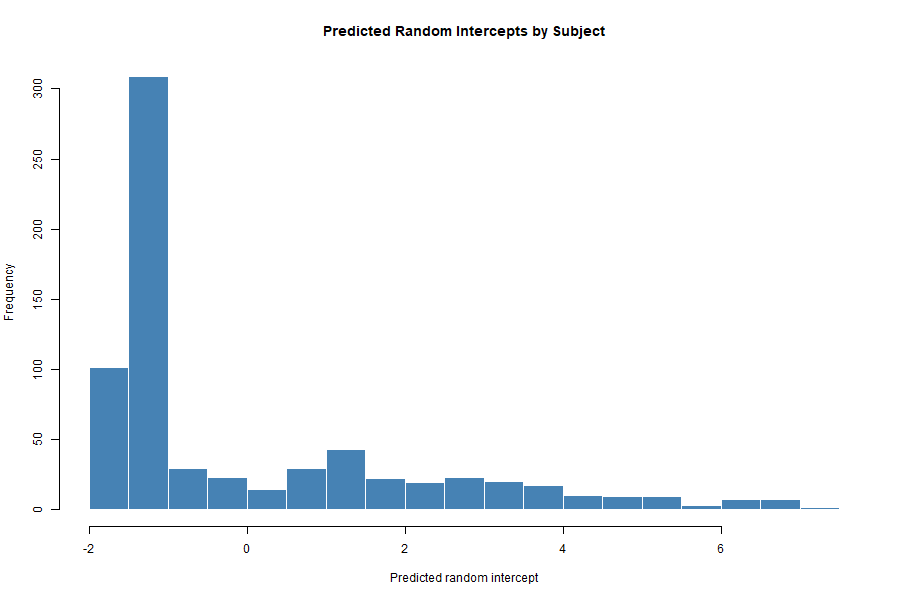
\includegraphics[width=0.75\textwidth]{../hw7_code/output/glmm_random_intercept_histogram.png}
\caption{Histogram of predicted random intercepts from the GLMM.}
\label{fig:glmm-random-intercept-histogram}
\end{figure}

\begin{figure}[htbp]
\centering
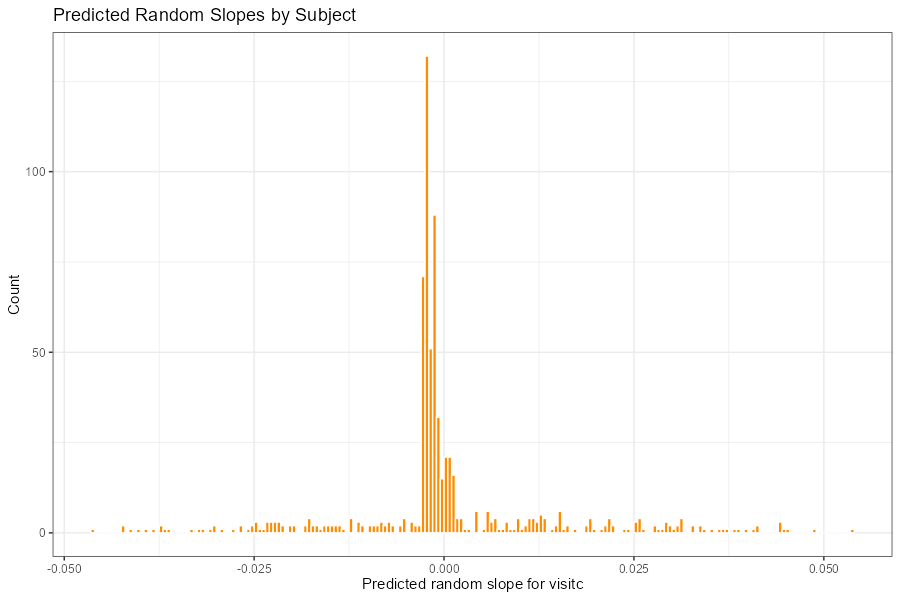
\includegraphics[width=0.75\textwidth]{../hw7_code/output/glmm_random_slope_histogram.png}
\caption{Histogram of predicted random slopes for visit time from the GLMM.}
\label{fig:glmm-random-slope-histogram}
\end{figure}

\subsection{Subject-specific probabilities}

For randomly selected subjects, predicted subject-specific probabilities of obstruction
over time are shown in \cref{fig:glmm-subject-probabilities}. These predictions
use both the fixed effect estimates and each subject's predicted random effects.


\begin{figure}[htbp]
\centering
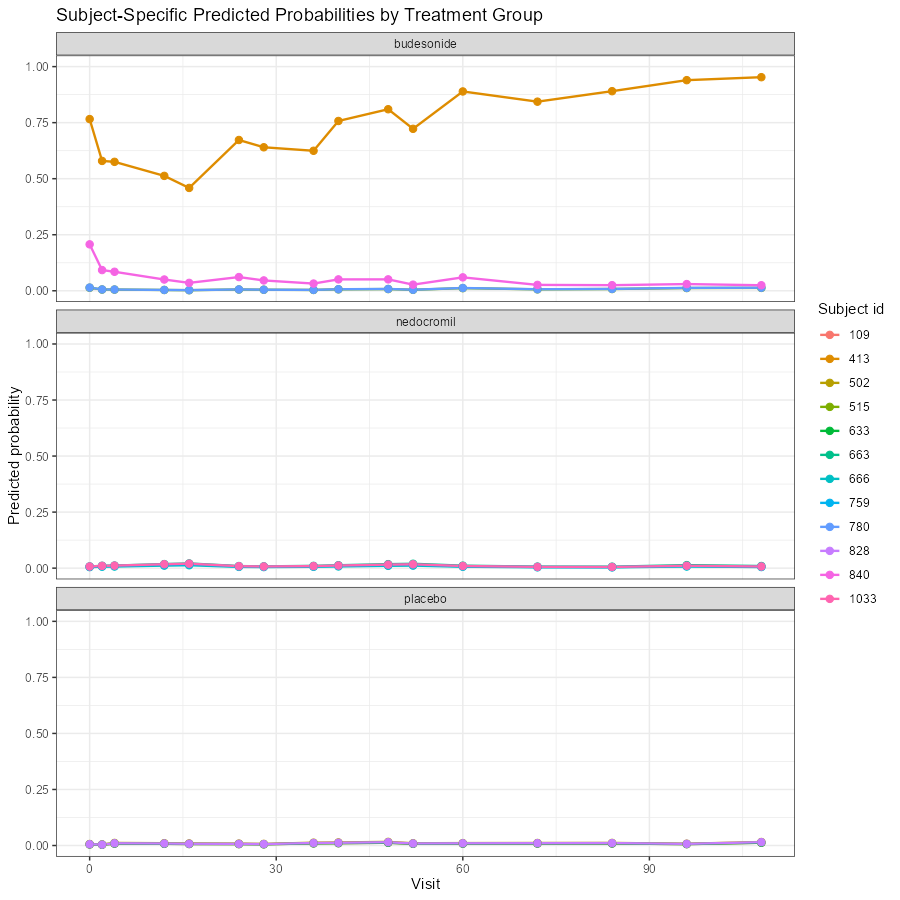
\includegraphics[width=0.9\textwidth]{../hw7_code/output/glmm_selected_subject_probabilities.png}
\caption{Predicted subject-specific probabilities of obstruction for selected subjects.}
\label{fig:glmm-subject-probabilities}
\end{figure}

\section{Summary}

We fit a logistic mixed effects model for pre-bronchodilator obstruction status, using fixed
effects for treatment group, categorical visit time, treatment-by-visit interaction,
age at randomization, gender, and ethnicity. The random-effects
structure included both a subject-specific random intercept and a
subject-specific random slope for continuous visit time.

There is evidence that the subject-specific obstruction trajectories differ by
treatment group. The random effects also show meaningful between-subject
heterogeneity, especially in baseline obstruction odds.

For this data, I would prefer GLMM when the goal is subject-specific inference
or prediction. In addition, I would prefer GEE when the goal is population-average inference
or prediction.

\section{Code Availability}

The code is available at
\url{https://github.com/CHENGHAO-WANG/767_homework/tree/main/hw7_code}.

\end{document}
